\section{Übersicht der Systemarchitektur}
\begin{figure}[h]
    \centering
    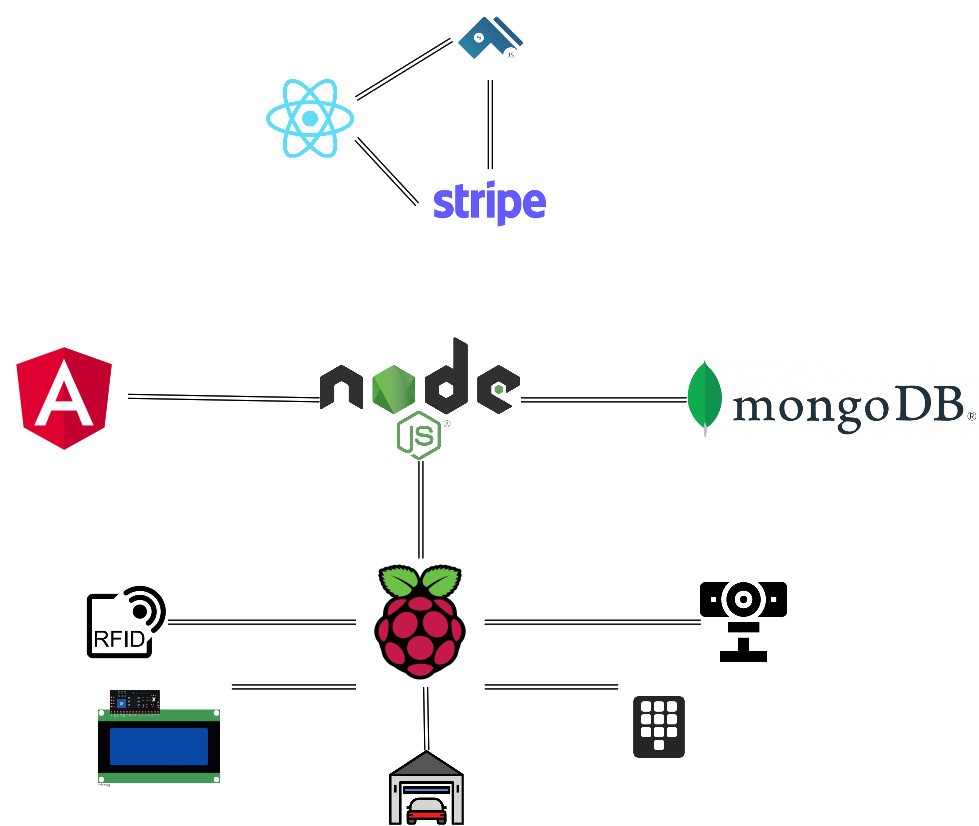
\includegraphics[width=10cm]{pics/APERTASystemarchitektur.jpg}
    \caption{Systemarchitektur}
    \end{figure}
Diese Diplomarbeit setzt sich aus zwei voneinander unabhängigen Systemen zusammen. Das Shopsystem, bestehend aus einem React-Frontend, kommuniziert mit zwei Bibliotheken, CommerceJS und Stripe, welche für die Produktverwaltung, sowie den Bezahlvorgang zuständig sind. Das Angular-Frontend des Dashboard in Verbindung mit dem NodeJS Server, der MongoDB Datenbank sowie dem Raspberry bietet das zweite System.
Der Raspberry ist über GPIOs mit dem RFID-Leser, dem Nummernfeld und dem Display verbunden. Weiters wurde die Kamera an einen der USB 3.0 Ports des Raspberry angeschlossen.
\section{Frontend (Angular-Applikation)}
\setauthor{David Hauser}

\section{Frontend (React-Applikation)}
\setauthor{Benjamin Golic}
